\documentclass[a4paper,9pt]{extarticle}

%=========================================================
% PACKAGES
%=========================================================

\usepackage[
a4paper,
top=1.8cm,
bottom=1.5cm,
footskip=7mm,
left=1cm,
right=1cm,
headheight=14pt,
headsep=5mm
]{geometry}
\usepackage[T1]{fontenc}
\usepackage[utf8]{inputenc}
\usepackage[french]{babel}

\usepackage[sfdefault]{FiraSans}
\renewcommand{\familydefault}{\sfdefault}

\usepackage{multicol}
\setlength{\columnsep}{0.7cm}

\usepackage{amsmath,amssymb}

\usepackage{titlesec}
\usepackage{enumitem}

\usepackage{tcolorbox}
\tcbuselibrary{skins,breakable}

\usepackage{xcolor}

\usepackage{graphicx}
\usepackage{float}

\usepackage{tikz}

\usepackage{fancyhdr}
\usepackage[hidelinks]{hyperref}


%=========================================================
% PAGE SETTINGS
%=========================================================

\setlength{\parindent}{0pt}
\setlength{\parskip}{1.5pt}

\setlength{\abovedisplayskip}{4pt}
\setlength{\belowdisplayskip}{4pt}

\setlist[itemize]{
leftmargin=*,
itemsep=1pt,
topsep=1pt
}


%=========================================================
% COLORS
%=========================================================

\definecolor{Blue}{HTML}{E3F0FF}
\definecolor{Green}{HTML}{E3F7EA}
\definecolor{Pink}{HTML}{FFE5ED}
\definecolor{Orange}{HTML}{FFF0DC}
\definecolor{Purple}{HTML}{EEE7FF}
\definecolor{Yellow}{HTML}{FFFADB}


\definecolor{BlueTitle}{HTML}{285B8F}
\definecolor{GreenTitle}{HTML}{287052}
\definecolor{PinkTitle}{HTML}{A84063}
\definecolor{OrangeTitle}{HTML}{A96500}
\definecolor{PurpleTitle}{HTML}{6245A5}


%=========================================================
% HEADER
%=========================================================

\pagestyle{fancy}

\fancyhf{}

\fancyhead[L]{\small\textbf{Numerical Methods}}
\fancyhead[C]{\small GPU Architecture}
\fancyhead[R]{\small Week 06 --- 12-18/10/2026}

\fancyfoot[C]{\small\href{https://github.com/AlphaXT38G/notes_ba5}{github.com/AlphaXT38G/notes\_ba5}}
\fancyfoot[R]{\small \thepage}

\renewcommand{\headrulewidth}{0.4pt}



%=========================================================
% TITLES
%=========================================================

\titleformat{\section}
{\large\bfseries\color{BlueTitle}}
{}{0pt}{}

\titlespacing{\section}
{0pt}{6pt}{3pt}


% separator

\newcommand{\separator}{
\vspace{2pt}
\hrule
\vspace{3pt}
}


%=========================================================
% BOXES
%=========================================================

% Boxes are kept whole (unbreakable): inside multicols, a box split by tcolorbox
% leaves an empty column behind it.

% DEFINITION - blue
\newtcolorbox{definition}{
enhanced,
unbreakable,
colback=Blue,
colframe=BlueTitle,
boxrule=0.7pt,
arc=0mm,
title=\textbf{Definition},
fonttitle=\bfseries
}

% IMPORTANT - pink
\newtcolorbox{important}{
enhanced,
unbreakable,
colback=Pink,
colframe=PinkTitle,
boxrule=0.7pt,
arc=0mm,
title=\textbf{Key idea},
fonttitle=\bfseries
}

% FORMULAS - green
\newtcolorbox{formula}{
enhanced,
unbreakable,
colback=Green,
colframe=GreenTitle,
boxrule=0.7pt,
arc=0mm,
title=\textbf{Key formulas},
fonttitle=\bfseries
}

% WARNING - orange
\newtcolorbox{warning}{
enhanced,
unbreakable,
colback=Orange,
colframe=OrangeTitle,
boxrule=0.7pt,
arc=0mm,
title=\textbf{Warning},
fonttitle=\bfseries
}

% EXAMPLE - purple
\newtcolorbox{example}{
enhanced,
unbreakable,
colback=Purple,
colframe=PurpleTitle,
boxrule=0.7pt,
arc=0mm,
title=\textbf{Example},
fonttitle=\bfseries
}

% SUMMARY - orange
\newtcolorbox{summary}{
enhanced,
unbreakable,
colback=Yellow,
colframe=OrangeTitle,
boxrule=0.7pt,
arc=0mm,
title=\textbf{Summary},
fonttitle=\bfseries
}



%=========================================================
% FIGURE BOX
%=========================================================

\newtcolorbox{figurebox}{
enhanced,
colback=white,
colframe=gray,
boxrule=0.5pt,
arc=0mm,
center
}



%=========================================================
% DOCUMENT
%=========================================================

\begin{document}

%\footnotesize   --> To reduce the size of the text

\thispagestyle{fancy}



% Columns keep their natural height: boxes are unbreakable, stretching would open gaps.
\raggedcolumns
\begin{multicols}{2}


%=========================================================
\section{CPUs vs GPUs}


\begin{summary}

\begin{center}
\begin{tabular}{p{0.44\linewidth}|p{0.44\linewidth}}
\textbf{CPUs} (a cheetah) & \textbf{GPUs} (an army of snails) \\
\hline
Evolved to run single-threaded code as fast as possible &
Run massively parallel code \\
Nowadays: several cores ($\sim$4-16) for additional parallelization &
Must have 10K - millions of ``work items'' to use effectively \\
Optimize \textbf{latency} & Optimize \textbf{throughput} \\
\end{tabular}
\end{center}

\end{summary}


\begin{important}

\textbf{Learning goals}

\begin{itemize}

\item Understand how GPU cores differ from CPU cores.

\item Understand which workloads run better on GPUs vs CPUs.

\end{itemize}

\end{important}


\begin{example}

\textbf{3D graphics, then and now}

\begin{itemize}

\item Around 1996: Nintendo 64, 320$\times$400 pixels, 30 frames per second, runs at 62.5 MHz.

\item 2025 consumer GPUs: AMD RX 7900 XTX ($\sim$1K CHF), NVIDIA RTX 5090 ($\sim$2K CHF, the
card presented in detail below). Unreal Engine scenes.

\end{itemize}

\end{example}



%=========================================================
\section{Graphics is Brutal}


Rendering a triangle: a small program (\emph{shader}) computes the color of each pixel, e.g.\
load a texture value and multiply it by $\max(0, \texttt{dot(light\_dir, normal)})$. Compiled to
(hypothetical) machine instructions: \texttt{LOAD\_TEXTURE}, \texttt{MUL}, \texttt{FMA},
\texttt{FMA}, \texttt{MAX}, \texttt{MUL}, \texttt{MUL}, \texttt{MUL}.


\begin{formula}

\textbf{Modern requirements}

\begin{itemize}

\item 4K resolution (3840 $\times$ 2160 pixels), 60 frames per second

\item That's $\sim$\textbf{500 million} pixels per second\dots

\begin{itemize}

\item $\times$ the number of instructions to produce a color (complex shaders have many
more instructions)

\item $\times$ overdraw, multiple passes

\end{itemize}

\item Millions of triangles in the scene

\end{itemize}

Bottom line: \textbf{$\frac{1}{2}$ - $1\frac{1}{2}$ trillion operations per second}. Normal
processors can't keep up with that.

\end{formula}


\begin{definition}

\textbf{EMBARRASSINGLY PARALLEL PROBLEM}

Rendering is one: let's compute all the pixels in parallel.

\end{definition}


\begin{warning}

\textbf{Problem}: CPU-style processors are \textbf{too big}, we can only have a few. We will have
to make some tough compromises\dots

\end{warning}



%=========================================================
\section{From CPU to GPU}


\textbf{Review: CPU cores}

\begin{center}

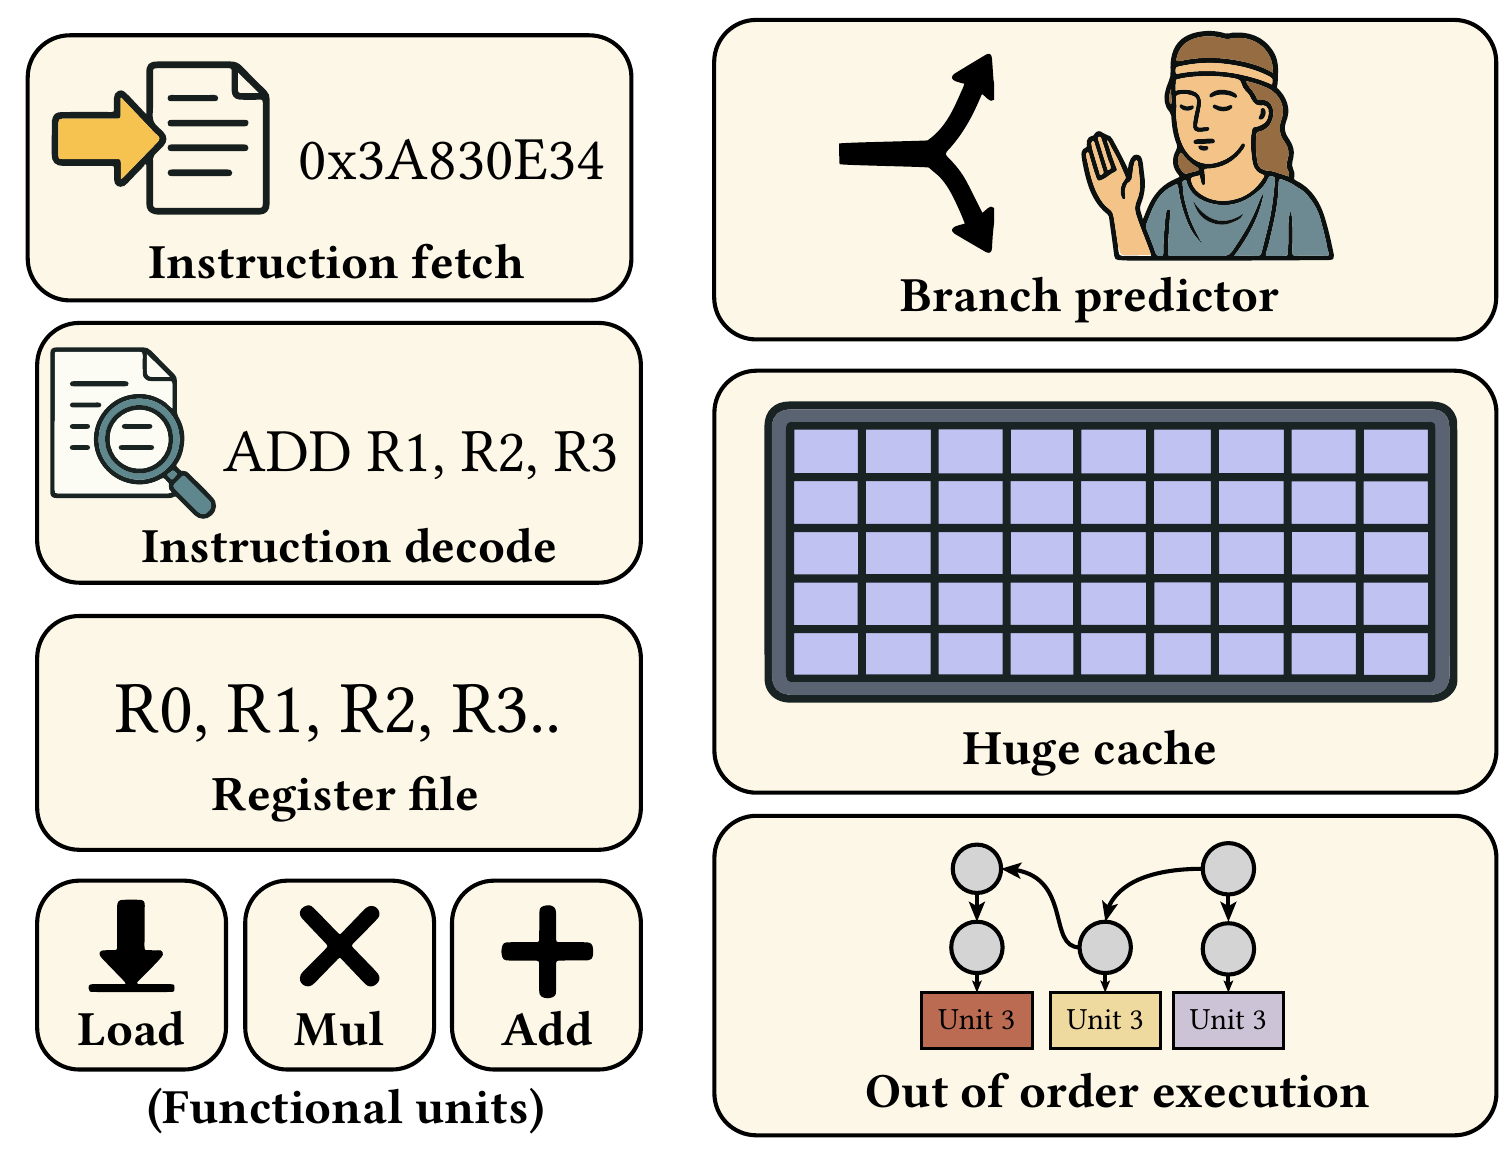
\includegraphics[
width=0.85\linewidth
]{../images/week06_01.png}

\end{center}


Left: what we \emph{want} to do (fetch, decode, register file, functional units). Right: what we
\emph{had} to do to make it fast (branch predictor, huge cache, out of order execution,
prefetcher).


\begin{important}

\textbf{Idea}: throw away all parts intended to make single-threaded programs run fast.

\end{important}


\begin{warning}

\textbf{Implications}

\begin{itemize}

\item Without branch predictor: every jump is slow.

\item Without out of order execution: an \texttt{ADD} waiting on a \texttt{LOAD} is slow.

\item Without big, fast caches: everything is slow.

\end{itemize}

\end{warning}


\begin{important}

When all pixels are computed in parallel, \textbf{all processors are evolving in lockstep}
(same instructions on different data). Let's exploit this in the architecture.

\end{important}



%=========================================================
\section{SM Partitions and Streaming Multiprocessors}


\begin{definition}

\textbf{SM PARTITION}

\textbf{32 tiny ``processors''} (each with its own register file and functional units: load,
mul, add) \textbf{sharing one instruction fetch + decode}. Similar to vector operations on CPUs.

\end{definition}


\begin{definition}

\textbf{STREAMING MULTIPROCESSOR (SM)}

4 SM partitions sharing an \textbf{L1 cache / shared memory} (128 KiB).

\end{definition}


\begin{center}

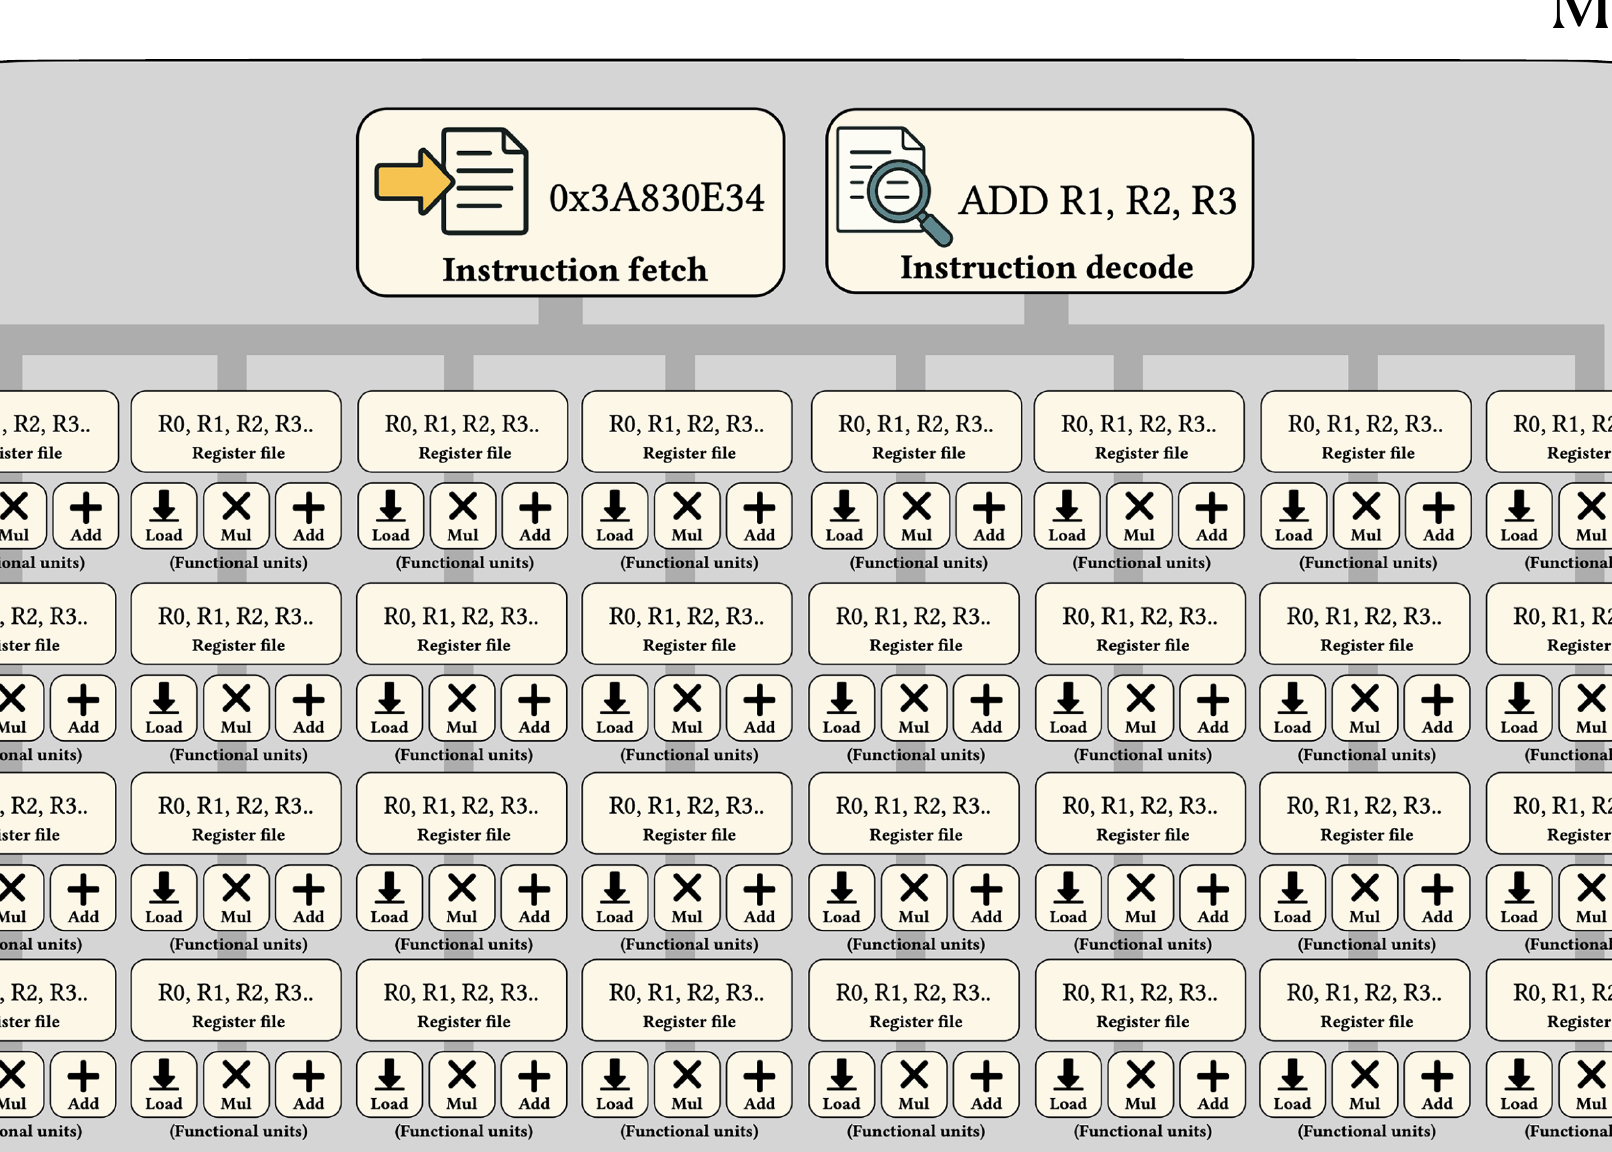
\includegraphics[
width=0.6\linewidth
]{../images/week06_02.png}

\end{center}


\begin{formula}

\textbf{NVIDIA RTX 5090} (Blackwell GB202 chip)

\begin{align*}
& 170 \text{ SMs} \times 4 \text{ partitions} \times 32 \text{ processing elements} \\
& =21'760 \text{ ``cores''}
\end{align*}

plus a \textbf{hardware scheduler}, an L2 cache (96 MiB) and the GPU memory (32 GiB).

\end{formula}



%=========================================================
\section{Design Choices}


Fast, complex circuit vs.\ slow, simple circuit: GPUs pick the second.


\begin{formula}

Latencies of different operations (approximate, worst case)

\begin{center}
\small
\begin{tabular}{l|cc}
 & RTX 5090 & Intel Core Ultra 9 285K \\
\hline
Clock frequency & 2.4 GHz & 5.7 GHz \\
Load (L1 hit) & 30 cycles & 4 cycles \\
Load (L2 hit) & 200 cycles & 17 cycles \\
Load (Miss) & 800 cycles & 565 cycles \\
\end{tabular}
\end{center}

\end{formula}


\begin{important}

\textbf{Is that it?} Just a lot of small, slow processors? No: two more ideas, latency hiding
and shared memory.

\end{important}



%=========================================================
\section{Part 1: Latency Hiding}


\begin{definition}

\textbf{WARP}

A group of 32 threads, executed by an SM partition.

\end{definition}


\begin{center}

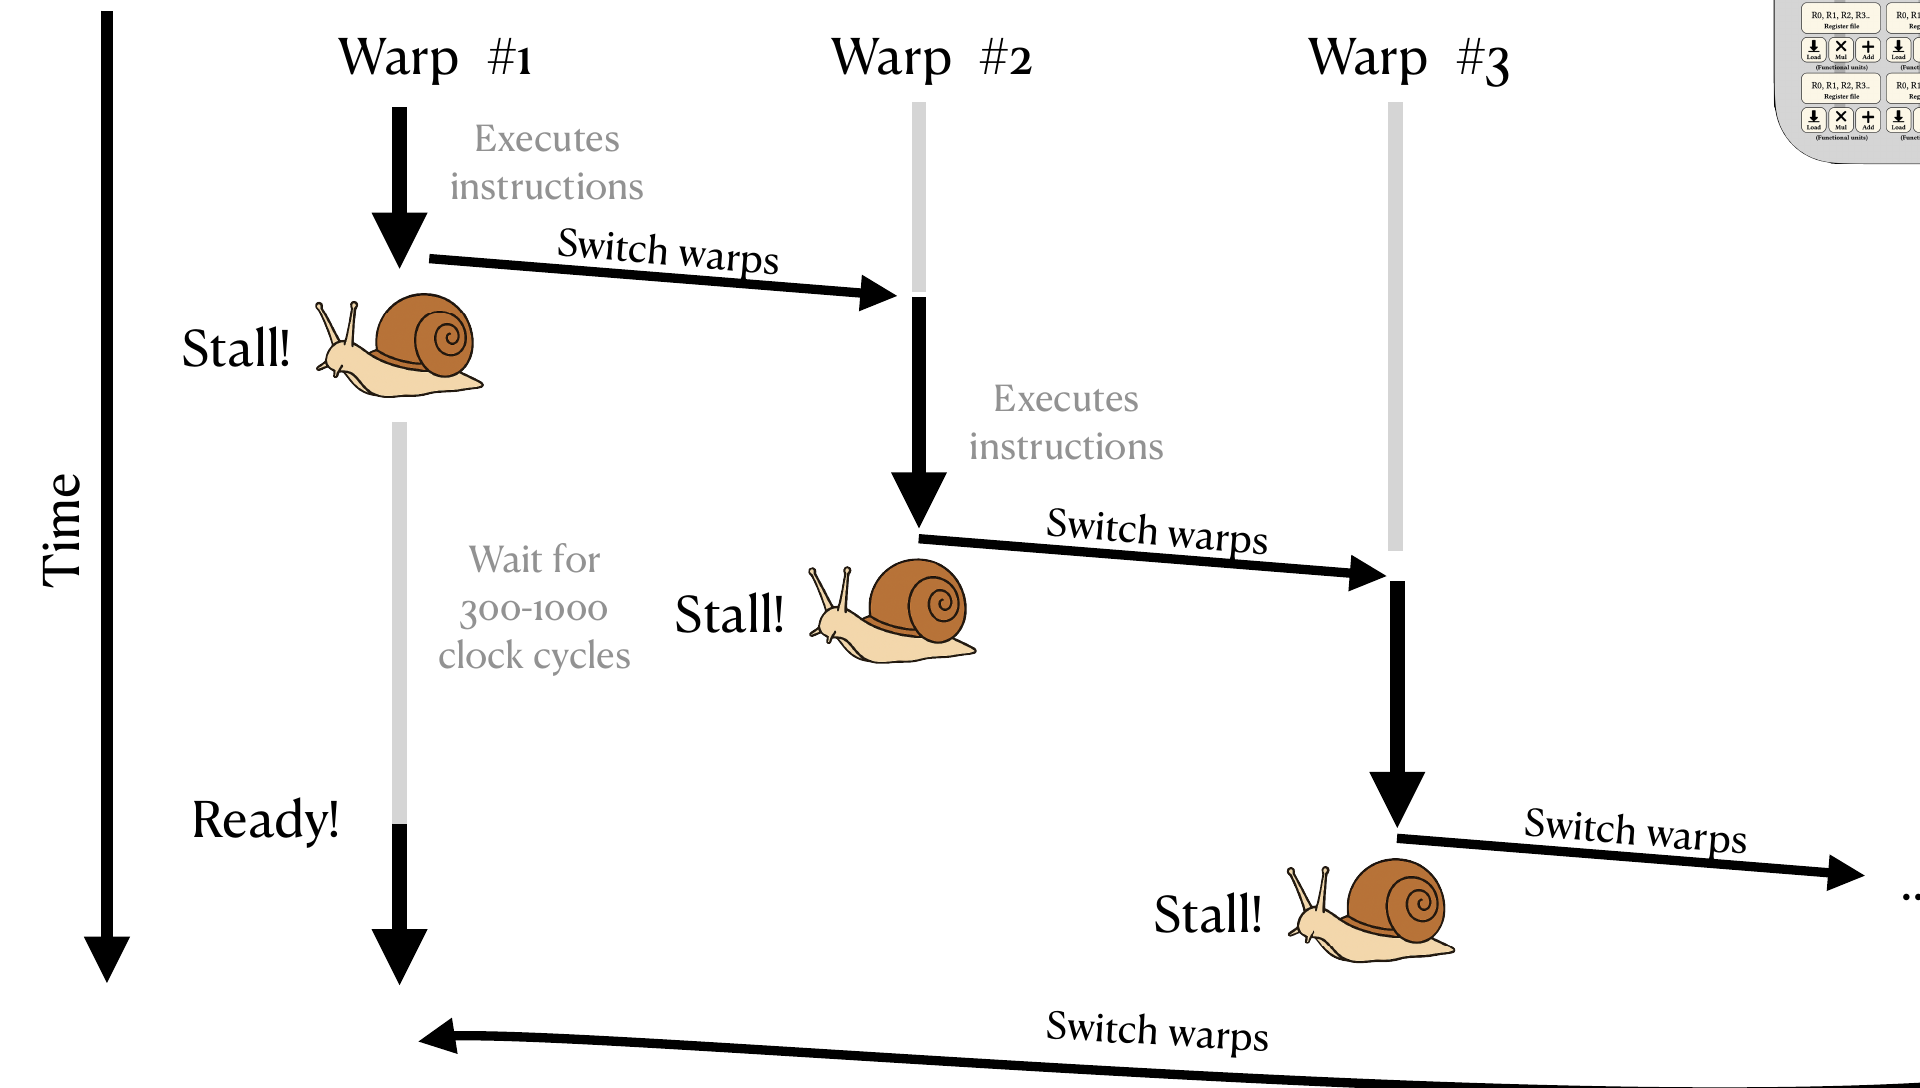
\includegraphics[
width=\linewidth
]{../images/week06_03.png}

\end{center}


\begin{important}

\begin{itemize}

\item Because the cores on GPUs are so basic, they will \textbf{stall all the time}; latencies
from stalls are \emph{terrible} for performance.

\item Stalls are unavoidable, but GPUs can usually ``hide'' this latency.

\item Key idea: run \textbf{many} warps per SM partition (\textbf{huge register file}).

\begin{itemize}

\item Switch to another warp whenever a stall happens (a stalled warp waits for 300-1000
clock cycles).

\item Switching is ``for free'' (consumes no clock cycles).

\item If all goes well: do useful work at every clock cycle.

\end{itemize}

\item Follows the high level pattern: optimize \textbf{throughput}, not latency.

\end{itemize}

\end{important}



%=========================================================
\section{Part 2: Shared Memory}


\begin{warning}

Most programs read and write a lot of memory: on GPUs, this means that they will stall
constantly.

\end{warning}


\begin{definition}

\textbf{SHARED MEMORY} (solution)

\begin{itemize}

\item Copy a small part of the problem into local (``shared'') memory.

\item Do \textbf{a lot of work} with this copy, which is fast to access.

\item Then write back the result.

\end{itemize}

\end{definition}



%=========================================================
\section{GPUs as Compute Accelerators}


\begin{definition}

\textbf{KERNEL}

You cannot run a browser or an operating system on a GPU: it merely helps to accelerate tasks.
Its basic computational unit is called a \textbf{kernel} (the CPU asks: ``Please run kernel
\texttt{matmul\_fp16\_1024}'', the GPU: ``OK!'').

\end{definition}


\begin{definition}

\textbf{KERNEL LAUNCH}

Code + a \textbf{launch grid}: the grid specifies how many instances of the program to launch,
e.g.\ $128 \times 128 \times 32$ times.

\end{definition}


\begin{example}

\textbf{GPUs for general purpose computing}

\begin{itemize}

\item Originally, GPUs could only render triangles. Main use: computer games!

\item People soon realized that their architecture is \emph{interesting} for non-graphics usage.

\item Hacky workarounds: full-screen rectangle + input data (as a texture) + graphics program =
output ``image'' (\emph{Brook for GPUs: Stream Computing on Graphics Hardware}, Buck et al.\
2004).

\item Today's frameworks make GPU programming easier: \textbf{CUDA} (NVIDIA), \textbf{ROCm}
(AMD), \textbf{SYCL} (Intel).

\end{itemize}

\end{example}



%=========================================================
\section{AI and Tensor Cores}


\begin{example}

\textbf{Developments in the last 5 years}: NVIDIA's stock price went up 1'202.17\%, currently
the most valuable company on earth (market capitalization). Not because of computer games:
datacenter GPUs ($\sim$50'000 CHF each) for \textbf{artificial intelligence}. GPUs are really,
really good at \textbf{matrix multiplication}, the fundamental operation underlying AI.

\end{example}


\begin{definition}

\textbf{TENSOR CORE}

Fancy name for a \textbf{matrix multiplication unit}. Like an FMA (fused-multiply-add) machine
instruction:

\begin{itemize}

\item FMA: \texttt{D = A * B + C}

\item Tensor core: \texttt{D = A @ B + C}

\end{itemize}

Multiplies a fixed matrix size quickly (e.g.\ $256 \times 32$ @ $32 \times 256$).

\end{definition}


\begin{important}

\begin{itemize}

\item Nowadays most of the computational ``power'' of a GPU is in the tensor core.

\item Recent trend: very low precision floating point (16 bit $\to$ 8 bit $\to$ 4 bit
``floats'').

\end{itemize}

\end{important}


\begin{formula}

Percentage of FLOP/s in tensor core:

\begin{center}
\small
\begin{tabular}{l|ccc}
 & 16 bit & 8 bit & 4 bit \\
\hline
B200 (data center) & 98.4\% & 99.2\% & 99.6\% \\
RTX 5090 & 75.0\% & 87.49\% & 93.8\% \\
\end{tabular}
\end{center}

\end{formula}



\end{multicols}


\end{document}
